\documentclass[%
crop,%
tikz,%
convert={outext=.svg,command=\unexpanded{pdf2svg \infile\space../_static/\outfile}},%
multi=false%
]{standalone}%
\usepackage[utf8]{luainputenc}%
\usepackage[no-math]{fontspec}%
\defaultfontfeatures{%
    Numbers={OldStyle,Proportional},%
    Ligatures=TeX,%
    Extension=.ttf,%
}%
\setmainfont[%
UprightFont=*-Regular,%
ItalicFont=*-Italic,%
BoldFont=*-Bold,%
BoldItalicFont=*-BoldItalic,%
]{Raleway}%
\setsansfont[%
UprightFont=*-Regular,%
ItalicFont=*-Italic,%
BoldFont=*-Bold,%
BoldItalicFont=*-BoldItalic,%
]{Raleway}%
\usepackage[frenchmath]{mathastext}%
\usepackage{amsmath}%
\usepackage{amssymb}%
\usepackage{mathrsfs}%
\usepackage{mathtools}%
\usepackage{siunitx}%
\usepackage[siunitx]{circuitikz}%
\usetikzlibrary{calc,backgrounds,arrows.meta,patterns}%

\DeclareMathOperator{\sign}{sign}%

% Ensembles
\let\C\relax
\newcommand{\R}{\ensuremath{\mathbb{R}}} % Réel
\newcommand{\N}{\ensuremath{\mathbb{N}}} % Entiers naturels
% \newcommand{\C}{\ensuremath{\mathbb{C}}} % Complexes
\newcommand{\B}{\ensuremath{\mathscr{B}}} % Bus électriques
\newcommand{\Ch}{\ensuremath{\mathscr{C}}} % Charges
\renewcommand{\L}{\ensuremath{\mathscr{L}}} % Lignes
\renewcommand{\P}{\ensuremath{\mathscr{P}}} % Phases

% Phases
\newcommand{\arm}{\ensuremath{\mathrm{a}}}%
\newcommand{\brm}{\ensuremath{\mathrm{b}}}%
\newcommand{\crm}{\ensuremath{\mathrm{c}}}%
\newcommand{\nrm}{\ensuremath{\mathrm{n}}}%
\newcommand{\trm}{\ensuremath{\mathrm{t}}}%
\newcommand{\grm}{\ensuremath{\mathrm{g}}}%
\newcommand{\abrm}{\ensuremath{\mathrm{ab}}}%
\newcommand{\bcrm}{\ensuremath{\mathrm{bc}}}%
\newcommand{\carm}{\ensuremath{\mathrm{ca}}}%
\newcommand{\anrm}{\ensuremath{\mathrm{an}}}%
\newcommand{\bnrm}{\ensuremath{\mathrm{bn}}}%
\newcommand{\cnrm}{\ensuremath{\mathrm{cn}}}%
\newcommand{\atrm}{\ensuremath{\mathrm{at}}}%
\newcommand{\btrm}{\ensuremath{\mathrm{bt}}}%
\newcommand{\ctrm}{\ensuremath{\mathrm{ct}}}%
\newcommand{\ntrm}{\ensuremath{\mathrm{nt}}}%
\newcommand{\agrm}{\ensuremath{\mathrm{ag}}}%
\newcommand{\bgrm}{\ensuremath{\mathrm{bg}}}%
\newcommand{\cgrm}{\ensuremath{\mathrm{cg}}}%
\newcommand{\ngrm}{\ensuremath{\mathrm{ng}}}%
\newcommand{\abcrm}{\ensuremath{\mathrm{abc}}}%
\newcommand{\abcnrm}{\ensuremath{\mathrm{abcn}}}%

% Indices ou exposants
\newcommand{\cons}{\ensuremath{\mathrm{cons.}}}%
\renewcommand{\prod}{\ensuremath{\mathrm{prod.}}}%
\newcommand{\theo}{\ensuremath{\mathrm{th.}}}%
\newcommand{\const}{\ensuremath{\mathrm{const.}}}%

% Variables
\newcommand{\umax}{\ensuremath{U^{\max}}}%
\newcommand{\umaxnorm}{\ensuremath{U^{\max\,\text{norm.}}}}%
\newcommand{\umin}{\ensuremath{U^{\min}}}%
\newcommand{\uminnorm}{\ensuremath{U^{\min\,\text{norm.}}}}%
\newcommand{\unom}{\ensuremath{U^{\text{nom.}}}}%
\newcommand{\unomnorm}{\ensuremath{U^{\text{nom.}\,\text{norm.}}}}%
\newcommand{\uup}{\ensuremath{U^{\text{up}}}}%
\newcommand{\uupnorm}{\ensuremath{U^{\text{up}\,\text{norm.}}}}%
\newcommand{\uupprime}{\ensuremath{U^{\text{up}\,\prime}}}%
\newcommand{\udown}{\ensuremath{U^{\text{down}}}}%
\newcommand{\udownnorm}{\ensuremath{U^{\text{down}\,\text{norm.}}}}%
\newcommand{\udownprime}{\ensuremath{U^{\text{down}\,\prime}}}%
\newcommand{\smax}{\ensuremath{S^{\max}}}%
\newcommand{\pmax}{\ensuremath{P^{\max}}}%
\newcommand{\sproj}{\ensuremath{\underline{S^{\text{proj.}}}}}%
%

\begin{document}
    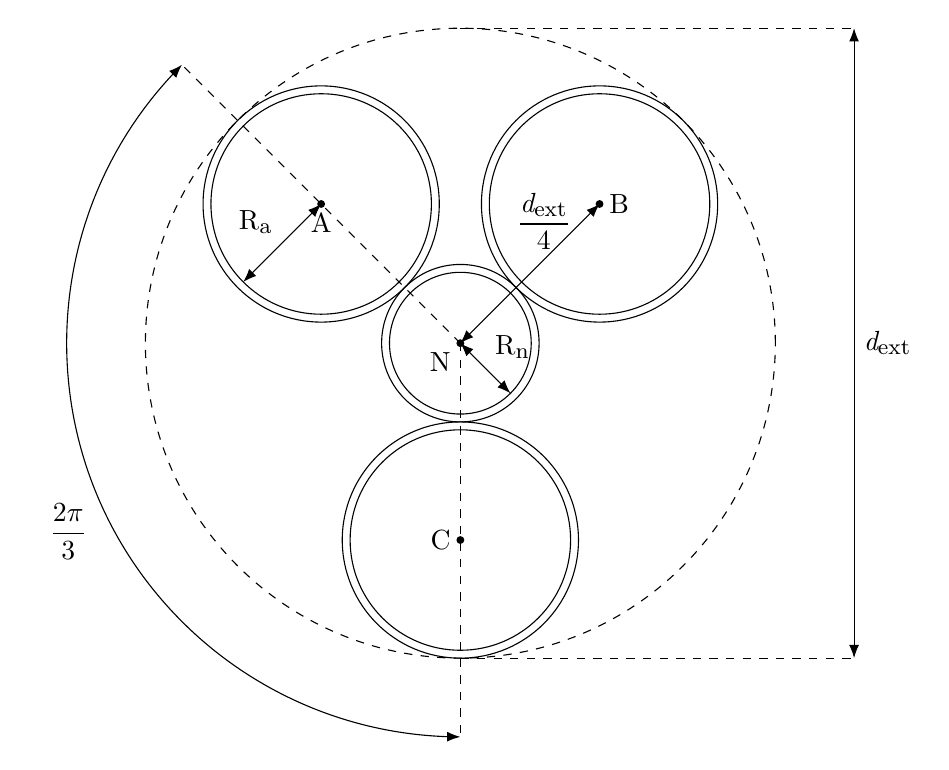
\begin{tikzpicture}[%
        show background rectangle,%
        tight background,%
        background rectangle/.style={fill=white}%
    ]
        \tikzset{%
            point/.pic={%
                \fill[black] (0,0) circle[radius=0.05];%
            }%
        }%

        %
        % Conducteurs
        %
        % Neutre
        \coordinate (neutral center) at (0,8);%
        \draw (neutral center) pic {point} node [below left] {N};%
        \draw (neutral center) circle[radius=1];%
        \draw (neutral center) circle[radius=0.90];%

        % Phases
        \foreach \x/\y/\z/\p in {a/135/A/below,b/45/B/right,c/-90/C/left} {%
            \path (neutral center) ++(\y:2.5) coordinate (\x\space center);%
            \draw (\x\space center) pic {point} node[\p] {\z};%
            \draw (\x\space center) circle[radius=1.5];%
            \draw (\x\space center) circle[radius=1.4];%
        }%
        \draw[dashed] (neutral center) circle[radius=4];%

        %
        % Annotations
        %
        % Exterior diameter
        \draw[{Latex[]}-{Latex[]}] (neutral center) ++(5,-4)%
        coordinate (bottom dext)%
        -- ++(0,8) coordinate(top dext)%
        node[midway, right] {$d_{\mathrm{ext}}$};%
        \draw[dashed] (neutral center) ++(0,4) -- (top dext);%
        \draw[dashed] (neutral center) ++(0,-4) -- (bottom dext);%

        % External diameter divided by 4
        \draw[{Latex[]}-{Latex[]}] (neutral center) -- (b center) %
        node [pos=0.6, above] {$\dfrac{d_{\mathrm{ext}}}{4}$};%

        % Arc
        \draw[dashed] (neutral center) -- ++(0,-5);%
        \draw[dashed] (neutral center) -- ++(135:5) coordinate (start arc);%
        \draw[{Latex[]}-{Latex[]}] (start arc) arc[start angle=135, end angle=270, radius=5]%
        node [midway, below left] {$\dfrac{2\pi}{3}$};%

        % Radius neutral
        \draw[{Latex[]}-{Latex[]}] (neutral center) -- ++(-45:0.9) node[midway, above right] {$R_{\nrm}$};%

        % Radius phase
        \draw[{Latex[]}-{Latex[]}] (a center) -- ++(-135:1.4) node[midway, above left] {$R_{\arm}$};%
    \end{tikzpicture}
\end{document}
% Local Variables:
% mode: latex
% TeX-engine: luatex
% TeX-source-correlate-method-active: synctex
% ispell-local-dictionary: "british"
% coding: utf-8
% LaTeX-indent-level: 4
% fill-column: 120
% End:
